\documentclass[journal,12pt,onecolumn]{IEEEtran}
\usepackage{cite}
 \usepackage{caption}
\usepackage{graphicx}
\usepackage{amsmath,amssymb,amsfonts,amsthm}
\usepackage{algorithmic}
\usepackage{graphicx}
\usepackage{textcomp}
\usepackage{xcolor}
\usepackage{txfonts}
\usepackage{listings}
\usepackage{enumitem}
\usepackage{mathtools}
\usepackage{gensymb}
\usepackage{comment}
\usepackage[breaklinks=true]{hyperref}
\usepackage{tkz-euclide} 
\usepackage{listings}
\usepackage{gvv}                                        
%\def\inputGnumericTable{}                                 
\usepackage[latin1]{inputenc} 
\usetikzlibrary{arrows.meta, positioning}
\usepackage{xparse}
\usepackage{color}                                            
\usepackage{array}                                            
\usepackage{longtable}                                       
\usepackage{calc}                                             
\usepackage{multirow}
\usepackage{multicol}
\usepackage{hhline}                                           
\usepackage{ifthen}                                           
\usepackage{lscape}
\usepackage{tabularx}
\usepackage{array}
\usepackage{float}
\newtheorem{theorem}{Theorem}[section]
\newtheorem{problem}{Problem}
\newtheorem{proposition}{Proposition}[section]
\newtheorem{lemma}{Lemma}[section]
\newtheorem{corollary}[theorem]{Corollary}
\newtheorem{example}{Example}[section]
\newtheorem{definition}[problem]{Definition}
\newcommand{\BEQA}{\begin{eqnarray}}
\newcommand{\EEQA}{\end{eqnarray}}
\usepackage{float}
%\newcommand{\define}{\stackrel{\triangle}{=}}
\theoremstyle{remark}
\usepackage{circuitikz}
\captionsetup{justification=centering}
\usepackage{tikz}
\title{EC: ELECTRONICS AND COMMUNICATION ENGINEERING - 2017}
\author{EE25BTECH11037 - Divyansh}


\begin{document}
\maketitle

\begin{enumerate}

\item Consider the $5 \times 5$ matrix  
$
A = \myvec{1 & 2 & 3 & 4 & 5 \\
5 & 1 & 2 & 3 & 4 \\
4 & 5 & 1 & 2 & 2 \\
3 & 4 & 5 & 1 & 2 \\
2 &3 & 4 & 5 & 1}
$ 
It is given that $A$ has only one real eigenvalue. Then the real eigenvalue of $A$ is  
\begin{multicols}{4}
\begin{enumerate}
\item $-2.5$
\item $0$
\item $15$
\item $25$
\end{enumerate}
\end{multicols}
\hfill \brak{\text{GATE EC 2017}}

\item The rank of the matrix 
$
M = \begin{bmatrix}
5 & 10 & 10 \\
1 & 0 & 2 \\
3 & 6 & 6
\end{bmatrix}
$ is  
\begin{multicols}{4}
\begin{enumerate}
\item $0$
\item $1$
\item $2$
\item $3$
\end{enumerate}
\end{multicols}
\hfill \brak{\text{GATE EC 2017}}

\item Consider the following statements about the linear dependence of the real-valued functions $y_1 = 1$, $y_2 = x$, and $y_3 = x^2$, over the field of real numbers:  
\begin{enumerate}[label=\Roman*.]
    \item $y_1$, $y_2$, $y_3$ are linearly independent on $-1 \leq x \leq 0$ 
    \item $y_1$, $y_2$, $y_3$ are linearly dependent on $0 \leq x \leq 1$
    \item $y_1$, $y_2$, $y_3$ are linearly independent on $0 \leq x \leq 1$
    \item $y_1$, $y_2$, $y_3$ are linearly dependent on $-1 \leq x \leq 0$
\end{enumerate}
 
Which one among the following is correct?  
\begin{multicols}{2}
\begin{enumerate}
\item Both I and II are true
\item Both I and III are true
\item Both II and IV are true
\item Both III and IV are true
\end{enumerate}
\end{multicols}
\hfill \brak{\text{GATE EC 2017}}

\item Three fair cubical dice are thrown simultaneously. The probability that all three dice have the same number of dots on the faces showing up is \brak{\text{up to third decimal place}} $\underline{\hspace{1cm}}$.

\hfill \brak{\text{GATE EC 2017}}

\item Consider the following statements for continuous-time linear time invariant \brak{LTI} systems:  
\begin{enumerate}[label=\Roman*.]
    \item There is no bounded input bounded output \brak{BIBO} stable system with a pole in the right half of the complex plane.
    \item There is no causal and BIBO stable system with a pole in the right half of the complex plane.  
\end{enumerate}

Which one among the following is correct?  
\begin{multicols}{2}
\begin{enumerate}
\item Both I and II are true
\item Both I and II are not true
\item Only I is true
\item Only II is true
\end{enumerate}
\end{multicols}
\hfill \brak{\text{GATE EC 2017}}

\item Consider a single input single output discrete-time system with $x\sbrak{n}$ as input and $y\sbrak{n}$ as output, where the two are related as  

$
y\sbrak{n} = \begin{cases}
x\sbrak{n}, & 0 \leq n \leq 10 \\
x\sbrak{n} - x\sbrak{n-1}, & \text{otherwise}
\end{cases}
$
  
Which one of the following statements is true about the system?  
\begin{multicols}{2}
\begin{enumerate}
\item It is causal and stable
\item It is causal but not stable
\item It is not causal but stable
\item It is neither causal nor stable
\end{enumerate}
\end{multicols}
\hfill \brak{\text{GATE EC 2017}}

\item In the circuit shown in the $\figref{fig:placeholder_1}$, the positive angular frequency $\omega$ \brak{\text{in radians per second}} at which the magnitude of the phase difference between the voltages $V_1$ and $V_2$ equals $-\frac{\pi}{4}$ is  $\underline{\hspace{2cm}}$
\begin{figure}[H]
    \centering
    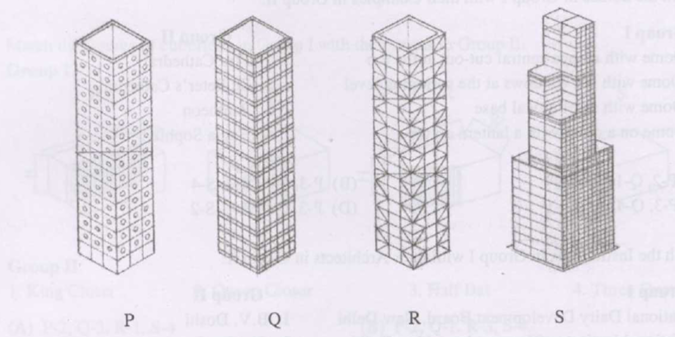
\includegraphics[width=0.5\columnwidth]{figs/2.png}
    \caption{\centering for q-7}
    \label{fig:placeholder_1}
\end{figure}

\hfill \brak{\text{GATE EC 2017}}

\item A periodic signal $x\brak{t}$ has a trigonometric Fourier series expansion  

\begin{align*}
    x\brak{t} = a_0 + \sum_{n=1}^{\infty} \brak{ a_n \cos\brak{n\omega_0 t}} + b_n \sin\brak{n\omega_0 t} )
\end{align*}

If $x\brak{t} = -x\brak{-t} = -x\brak{t - \frac{T}{2}}$, we can conclude that  
\begin{enumerate}
\item $a_n = 0$ for all $n$, and $b_n = 0$ for even $n$
\item $a_n = 0$ for all $n$, and $b_n = 0$ for odd $n$
\item $a_n = 0$ for even $n$, and $b_n = 0$ for odd $n$
\item $a_n = 0$ for odd $n$, and $b_n = 0$ for even $n$
\end{enumerate}
\hfill \brak{\text{GATE EC 2017}}

\item A bar of Gallium Arsenide \brak{GaAs} is doped with Silicon such that the Silicon atoms occupy Gallium and Arsenic sites in the GaAs crystal. Which one of the following statements is true?  
\begin{enumerate}
\item Silicon atoms act as p-type dopants in Arsenic sites and n-type dopants in Gallium sites
\item Silicon atoms act as n-type dopants in Arsenic sites and p-type dopants in Gallium sites
\item Silicon atoms act as p-type dopants in Arsenic as well as Gallium sites
\item Silicon atoms act as n-type dopants in Arsenic as well as Gallium sites
\end{enumerate}
\hfill \brak{\text{GATE EC 2017}}

\item An $n^+-n$ Silicon device is fabricated with uniform and non-degenerate donor doping concentrations of $N_{D1} = 1 \times 10^{18} \text{cm}^{-3}$ and $N_{D2} = 1 \times 10^{15} \text{cm}^{-3}$ corresponding to the $n^+$ and $n$ regions respectively. At the operational temperature $T$, assume complete impurity ionization, $kT/q = 25 \text{mV}$, and intrinsic carrier concentration to be $n_i = 1 \times 10^{10} \text{cm}^{-3}$. What is the magnitude of the built-in potential of this device?  

\begin{multicols}{4}
\begin{enumerate}
\item $0.748 \text{V}$
\item $0.460 \text{V}$
\item $0.288 \text{V}$
\item $0.173 \text{V}$
\end{enumerate}
\end{multicols}
\hfill \brak{\text{GATE EC 2017}}

\item For a narrow base PNP BJT, the excess minority carrier concentrations \brak{denoted $\Delta n_E$, $\Delta p_B$, $\Delta n_C$} normalized to equilibrium minority carrier concentrations ($n_{E0}$, $p_{P0}$, $n_{C0}$) in the quasi-neutral emitter, base and collector regions are shown below in the $\figref{fig:placeholder_2}$. Which one of the following biasing modes is the transistor operating in?
\begin{figure}[H]
    \centering
    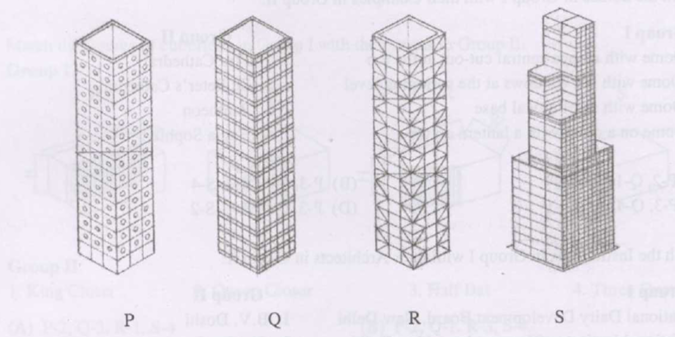
\includegraphics[width=0.5\columnwidth]{figs/2.png}
    \caption{\centering for q-11}
    \label{fig:placeholder_2}
\end{figure}
\begin{multicols}{4}
\begin{enumerate}
\item Forward active
\item Saturation
\item Inverse active
\item Cutoff
\end{enumerate}
\end{multicols}
\hfill \brak{\text{GATE EC 2017}}

\item For the operational amplifier circuit shown in the $\figref{fig:placeholder_3}$, the output saturation voltages are $\pm 15$ V. The upper and lower threshold voltages for the circuit are, respectively,
\begin{figure}[H]
    \centering
    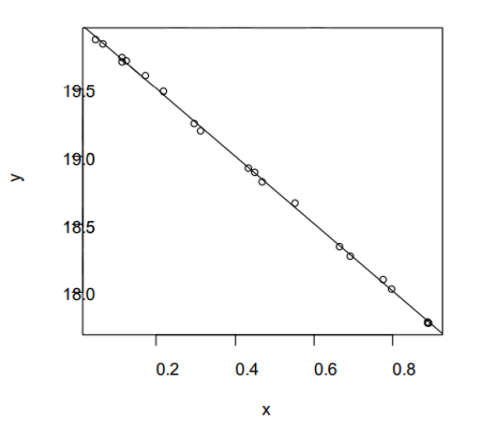
\includegraphics[width=0.5\columnwidth]{figs/3.png}
    \caption{\centering for q-12}
    \label{fig:placeholder_3}
\end{figure}
\begin{multicols}{4}
\begin{enumerate}
\item $+5$ V and $-5$ V
\item $+7$ V and $-3$ V
\item $+3$ V and $-7$ V
\item $+3$ V and $-3$ V
\end{enumerate}
\end{multicols}
\hfill \brak{\text{GATE EC 2017}}

\item A good transconductance amplifier should have
\begin{enumerate}
\item High input resistance and low output resistance
\item Low input resistance and high output resistance
\item High input and output resistances
\item Low input and output resistances
\end{enumerate}
\hfill \brak{\text{GATE EC 2017}}

\item The Miller effect in the context of a Common Emitter amplifier explains

\begin{enumerate}
\item An increase in the low-frequency cutoff frequency
\item An increase in the high-frequency cutoff frequency
\item A decrease in the low-frequency cutoff frequency
\item A decrease in the high-frequency cutoff frequency
\end{enumerate}
\hfill \brak{\text{GATE EC 2017}}

\item In the latch circuit shown in the $\figref{fig:placeholder_4}$, the NAND gates have non-zero, but unequal propagation delays. The present input condition is: $P = Q = 0$. If the input condition is changed simultaneously to $P = Q = 1$, the outputs $X$ and $Y$ are
\begin{figure}[H]
    \centering
    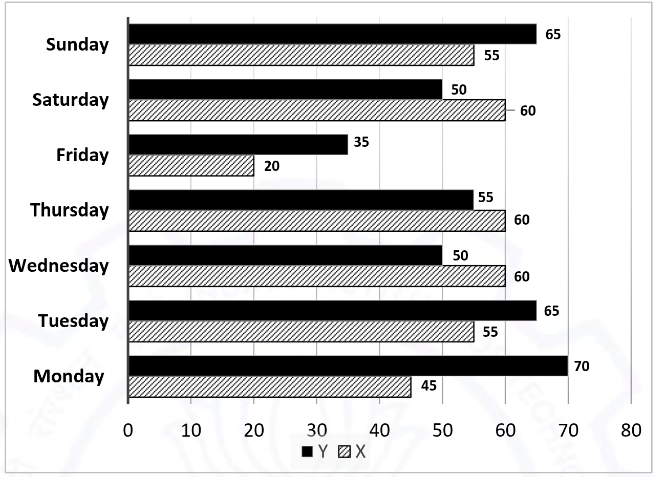
\includegraphics[width=0.5\columnwidth]{figs/4.png}
    \caption{\centering for q-15}
    \label{fig:placeholder_4}
\end{figure}
\begin{multicols}{2}
\begin{enumerate}
\item $X =  1$, $Y = 1$
\item Either $X = 1$, $Y = 0$ or $X = 0$, $Y = 1$
\item Either $X = 1$, $Y = 1$ or $X = 0$, $Y = 0$
\item $X = 0$, $Y = 0$
\end{enumerate}
\end{multicols}
\hfill \brak{\text{GATE EC 2017}}

\item The clock frequency of an $8085$ microprocessor is $5 MHz$. If the time required to execute an instruction is $1.4$ $\mu s$, then the number of T-states needed for executing the instruction is

\begin{multicols}{4}
\begin{enumerate}
\item $1$
\item $6$
\item $7$
\item $8$
\end{enumerate}
\end{multicols}
\hfill \brak{\text{GATE EC 2017}}

\item Consider the D-Latch shown in the $\figref{fig:placeholder_5}$, which is transparent when its clock input CK is high and has zero propagation delay. In the figure, the clock signal CLK1 has a $50\%$ duty cycle and CLK2 is a one-fifth period delayed version of CLK1. The duty cycle at the output of the latch in percentage is $\underline{\hspace{2cm}}$.
\begin{figure}[H]
    \centering
    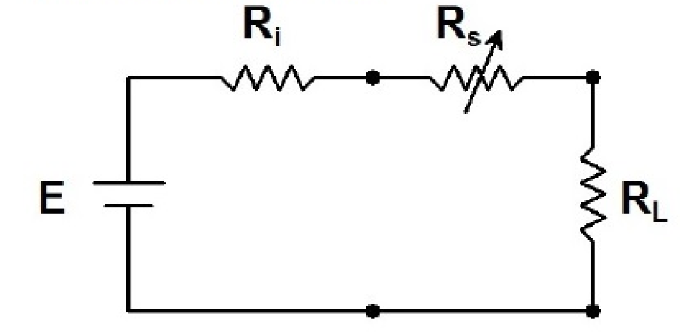
\includegraphics[width=0.5\columnwidth]{figs/5.png}
    \caption{\centering for q-17}
    \label{fig:placeholder_5}
\end{figure}

\hfill \brak{\text{GATE EC 2017}}

\item The open loop transfer function $G\brak{s} = \frac{K}{s\brak{s+2}\brak{s+3}\brak{s+1}}$ is connected in unity feedback configuration. Given that the steady state error is zero for unit step input and is $6$ for unit ramp input, the value of the parameter $K$ is $\underline{\hspace{2cm}}$.
\begin{figure}[H]
    \centering
    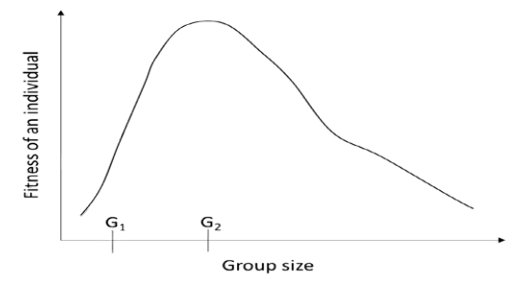
\includegraphics[width=0.5\columnwidth]{figs/6.png}
    \caption{\centering for q-18}
    \label{fig:placeholder_6}
\end{figure}

\hfill \brak{\text{GATE EC 2017}}

\item Consider a stable system with transfer function  
$G(s) = \dfrac{s^p + b_1 s^{p-1} + \dots + b_p}{s^q + a_1 s^{q-1} + \dots + a_q}$  
where $b_1, \dots, b_p$ and $a_1, \dots, a_q$ are real valued constants. The slope of the Bode log magnitude curve of $G\brak{s}$ converges to $-60$ dB/decade as $\omega \to \infty$. A possible pair of values for $p$ and $q$ is
\begin{multicols}{2}
\begin{enumerate}
\item $p = 0$, $q = 3$
\item $p = 1$, $q = 7$
\item $p = 2$, $q = 3$
\item $p = 3$, $q = 5$
\end{enumerate}
\end{multicols}
\hfill \brak{\text{GATE EC 2017}}

\item Which of the following can be the pole-zero configuration of a phase-lag controller \brak{\text{lag compensator}}?
\begin{figure}[H]
    \centering
    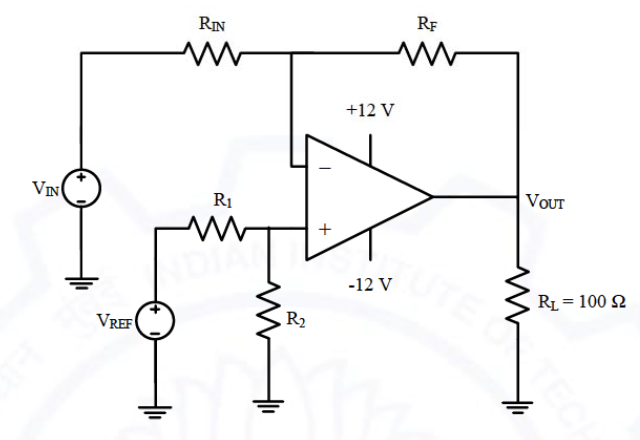
\includegraphics[width=0.9\columnwidth]{figs/7.png}
    \caption{\centering for q-20}
    \label{fig:placeholder_7}
\end{figure}

\hfill \brak{\text{GATE EC 2017}}

\item Let $\brak{X_1, X_2}$ be independent random variables. $X_1$ has mean $0$ and variance $1$, while $X_2$ has mean $1$ and variance $4$. The mutual information $I\brak{X_1; X_2}$ between $X_1$ and $X_2$ in bits is $\underline{\hspace{2cm}}$ . 

\hfill \brak{\text{GATE EC 2017}}

\item Which one of the following statements about differential pulse code modulation \brak{DPCM} is true?
\begin{enumerate}
\item The sum of message signal sample with its prediction is quantized
\item The message signal sample is directly quantized, and its prediction is not used
\item The difference of message signal sample and a random signal is quantized
\item The difference of message signal sample with its prediction is quantized
\end{enumerate}
\hfill \brak{\text{GATE EC 2017}}

\item In a digital communication system, the overall pulse shape $p\brak{t}$ at the receiver before the sampler has the Fourier transform $P\brak{f}$. If the symbols are transmitted at the rate of $2000$ symbols per second, for which of the following cases is the inter symbol interference zero?
\begin{figure}[H]
    \centering
    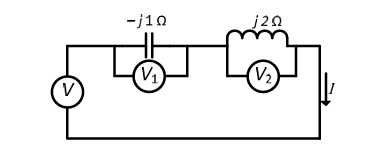
\includegraphics[width=0.8\columnwidth]{figs/8.png}
    \caption{\centering for q-23}
    \label{fig:placeholder_8}
\end{figure}

\hfill \brak{\text{GATE EC 2017}}

\item The voltage of an electromagnetic wave propagating in a coaxial cable with uniform characteristic impedance is $V\brak{l} = e^{-\gamma l + j\omega t}$ Volts, where $l$ is the distance along the length of the cable in metres, $\gamma = \brak{0.1 + j40}$ $m^{-1}$ is the complex propagation constant, and $\omega = 2\pi \times 10^9$ rad/s is the angular frequency. The absolute value of the attenuation in the cable in dB/metre is $\underline{\hspace{2cm}}$ . 

\hfill \brak{\text{GATE EC 2017}}

\item Consider a wireless communication link between a transmitter and a receiver located in free space, with finite and strictly positive capacity. If the effective areas of the transmitter and the receiver antennas, and the distance between them are all doubled, and everything else remains unchanged, the maximum capacity of the wireless link
\begin{multicols}{2}
\begin{enumerate}
\item Increases by a factor of $2$
\item Decreases by a factor of $2$
\item Remains unchanged
\item Decreases by a factor of $\sqrt{2}$
\end{enumerate}
\end{multicols}
\hfill \brak{\text{GATE EC 2017}}

\item Let $f\brak{x} = e^x + x$ for real $x$. From among the following, choose the Taylor series approximation of $f\brak{x}$ around $x = 0$, which includes all powers of $x$ less than or equal to $3$.
\begin{multicols}{2}
\begin{enumerate}
\item $1 + x + x^2 + x^3$
\item $1 + x + \frac{3}{2}x^2 + {x^3}$
\item $1 + x + \frac{3}{2}x^2 + \frac{7}{6}x^3$
\item $1 + x + 3x^2 + 7x^3$
\end{enumerate}
\end{multicols}
\hfill \brak{\text{GATE EC 2017}}

\item A three-dimensional region $R$ of finite volume is described by $x^2 + y^2 \leq z^3$, $0 \leq z \leq 1$, where $x$, $y$, $z$ are real. The volume of $R$ (up to two decimal places) is $\underline{\hspace{2cm}}$ .

\hfill \brak{\text{GATE EC 2017}}

\item Let $I = \int_C \brak{2z dx + 2ydy + 2xdz}$ where $x$, $y$, $z$ are real, and let $C$ be the straight line segment from point $A: \brak{0, 2, 1}$ to point $B: \brak{4, 1, -1}$. The value of $I$ is $\underline{\hspace{2cm}}$.

\hfill \brak{\text{GATE EC 2017}}

\item Which one of the following is the general solution of the first order differential equation $\frac{dy}{dx} = \brak{x + y - 1}^2$, where $x$, $y$ are real?
\begin{multicols}{2}
\begin{enumerate}
\item $y = 1 + x + \tan^{-1}\brak{x+c}$
\item $y = 1 + x + \tan\brak{x+c}$
\item $y = 1 - x + \tan^{-1}\brak{x+c}$
\item $y = 1 - x + \tan\brak{x+c}$
\end{enumerate}
\end{multicols}
\hfill \brak{\text{GATE EC 2017}}

\item Starting with $x = 1$, the solution of the equation $x^3 + x = 1$, after two iterations of Newton-Raphson's method $\brak{\text{up to two decimal places}}$ is $\underline{\hspace{2cm}}$.

\hfill \brak{\text{GATE EC 2017}}

\item Let $x\brak{t}$ be a continuous time periodic signal with fundamental period $T = 1$ seconds. Let $\cbrak{a_k}$ be the complex Fourier series coefficients of $x\brak{t}$, where $k$ is integer valued. Consider the following statements about $x\brak{3t}$:  
\begin{enumerate}[label=\Roman*.]
    \item The complex Fourier series coefficients of $x\brak{3t}$ are $\{a_k\}$ where $k$ is integer valued 
    \item The complex Fourier series coefficients of $x\brak{3t}$ are $\{3a_k\}$ where $k$ is integer valued
    \item The fundamental angular frequency of $x\brak{3t}$ is $6\pi$ rad/s 
\end{enumerate}
Which one of the following is correct?  
\begin{multicols}{2}
\begin{enumerate}
\item Only II and III are true
\item Only I and III are true
\item Only III is true
\item Only I is true
\end{enumerate}
\end{multicols}
\hfill \brak{\text{GATE EC 2017}}

\item Two discrete-time signals $x\sbrak{n}$ and $h\sbrak{n}$ are both non-zero only for $n = 0, 1, 2$, and are zero otherwise. It is given that $x\sbrak{0} = 1$, $x\sbrak{1} = 2$, $x\sbrak{2} = 1$, $h\sbrak{0} = 1$. Let $y\sbrak{n}$ be the linear convolution of $x\sbrak{n}$ and $h\sbrak{n}$. Given that $y\sbrak{1} = 3$ and $y\sbrak{2} = 4$, the value of the expression $(10y\sbrak{3} + y\sbrak{4})$ is
\begin{multicols}{4}
\begin{enumerate}
\item $31$
\item $32$
\item $33$
\item $34$
\end{enumerate}
\end{multicols}
\hfill \brak{\text{GATE EC 2017}}

\item Let $h\sbrak{n}$ be the impulse response of a discrete-time linear time invariant (LTI) filter. The impulse response is given by $h\sbrak{0} = 5$, $h\sbrak{1} = 1$, $h\sbrak{2} = -2$, and $h\sbrak{n} = 0$ for $n < 0$ and $n > 2$. Let $H\brak{\omega}$ be the discrete-time Fourier transform \brak{DTFT} of $h\sbrak{n}$, where $\omega$ is the normalized angular frequency in radians. Given that $H\brak{\omega_0} = 0$ and $0 < \omega_0 < \pi$, the value of $\omega_0$ \brak{\text{in radians}} is equal to
\begin{multicols}{4}
\begin{enumerate}
\item $\frac{\pi}{2}$
\item $\frac{2\pi}{3}$
\item $\frac{3\pi}{4}$
\item $\pi$
\end{enumerate}
\end{multicols}
\hfill \brak{\text{GATE EC 2017}}

\item The $\figref{fig:placeholder_9}$ shows an RLC circuit excited by the sinusoidal voltage $100 \cos\brak{3t}$ Volts, where $t$ is in seconds. The ratio $\dfrac{\text{amplitude of } V_2}{\text{amplitude of } V_1}$ is
\begin{figure}[H]
    \centering
    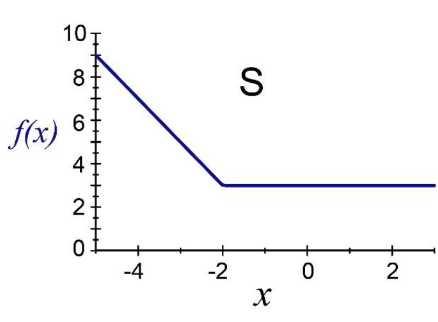
\includegraphics[width=0.5\columnwidth]{figs/9.png}
    \caption{\centering for q-34}
    \label{fig:placeholder_9}
\end{figure}
\begin{multicols}{4}
\begin{enumerate}
\item $2.5$
\item $2.6$
\item $2.7$
\item $2.8$
\end{enumerate}
\end{multicols}
\hfill \brak{\text{GATE EC 2017}}

\item In the circuit shown in the $\figref{fig:placeholder_10}$, the voltage $V_{\text{IN}}\brak{t}$ is described by:  
$V_{\text{IN}}\brak{t} = 0$, for $t < 0$  
$V_{\text{IN}}\brak{t} = 115$ Volts, for $t \geq 0$  
where $t$ is in seconds. The time \brak{\text{in seconds}} at which the current $I$ in the circuit will reach the value $2$ Amperes is $\underline{\hspace{2cm}}$
\begin{figure}[H]
    \centering
    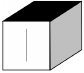
\includegraphics[width=0.5\columnwidth]{figs/10.png}
    \caption{\centering for q-35}
    \label{fig:placeholder_10}
\end{figure}

\hfill \brak{\text{GATE EC 2017}}

\item The dependence of drift velocity of electrons on electric field in a semiconductor is shown below in $\figref{fig:placeholder_11}$. The semiconductor has a uniform electron concentration of $n = 1 \times 10^{16}$ cm$^{-3}$ and electronic charge $q = 1.6 \times 10^{-19}$ C. If a bias of $5$ V is applied across a $1$ $\mu$m region of this semiconductor, the resulting current density in this region, in $ kA/cm$$^2$, is $\underline{\hspace{2cm}}$
\begin{figure}[H]
    \centering
    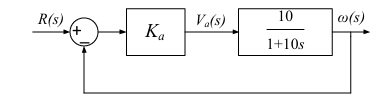
\includegraphics[width=0.5\columnwidth]{figs/11.png}
    \caption{\centering for q-36}
    \label{fig:placeholder_11}
\end{figure}

\hfill \brak{\text{GATE EC 2017}}

\item A uniformly doped Silicon bar of length $L = 0.1$ $\mu m $ with a donor concentration $N_D = 10^{16}$ $cm^{-3}$ is illuminated at $x = 0$ such that electron and hole pairs are generated at the rate of $G_L = G_0\brak{1 - x}$, $0 \leq x < L$, where $G_0 = 10^{17}$ cm$^{-3}$$s^{-1}$. Hole lifetime is $10^{-4}s$ , electronic charge $q = 1.6 \times 10^{-19} C $ , hole diffusion coefficient $D_p = 100$ $cm^2$/s and low level injection condition prevails. Assuming a linearly decaying steady state excess hole concentration that goes to $0$ at $x = L$, the magnitude of the diffusion current density at $x = L/2$, in $A/cm^2$, is $\underline{\hspace{2cm}}$
\begin{figure}[H]
    \centering
    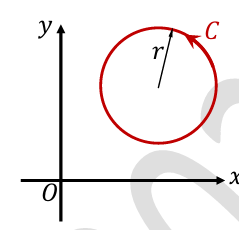
\includegraphics[width=0.5\columnwidth]{figs/12.png}
    \caption{\centering for q-37}
    \label{fig:placeholder_12}
\end{figure}
\hfill \brak{\text{GATE EC 2017}}

\item Two Silicon abrupt p-n junction diodes are fabricated with uniform donor doping concentrations of $N_{D1} = 10^{14}$ $cm^{-3}$ and $N_{D2} = 10^{16}$ $cm^{-3}$ in the n-regions of the diodes, and uniform acceptor doping concentrations of $N_{A1} = 10^{14}$ $cm^{-3}$ and $N_{A2} = 10^{16}$ $cm^{-3}$ in the p-regions of the diodes, respectively. Assuming that the reverse bias voltage is $\gg$ built-in potentials of the diodes, the ratio $C_2/C_1$ of their reverse bias capacitances for the same applied reverse bias, is $\underline{\hspace{2cm}}$
\begin{figure}[H]
    \centering
    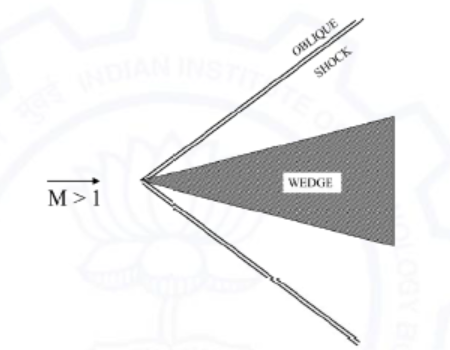
\includegraphics[width=0.5\columnwidth]{figs/13.png}
    \caption{\centering for q-38}
    \label{fig:placeholder_13}
\end{figure}

\hfill \brak{\text{GATE EC 2017}}

\item In the $\figref{fig:placeholder_14}$ shown, the npn transistor acts as a switch. For the input $V_{in}\brak{t}$ as shown in the figure, the transistor switches between the cut-off and saturation regions of operation, when $T$ is large. Assume collector-to-emitter voltage at saturation $V_{CE(\text{sat})} = 0.2 V$  and base-to-emitter voltage $V_{BE} = 0.7V$ . The minimum value of the common-base current gain $\alpha$ of the transistor for the switching should be $\underline{\hspace{2cm}}$.
\begin{figure}[H]
    \centering
    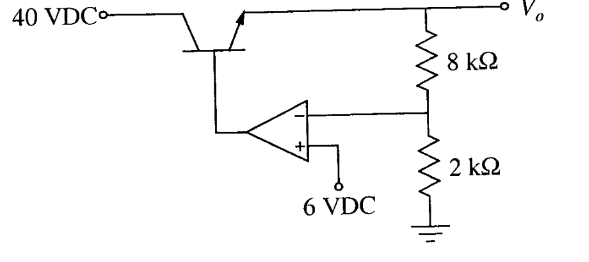
\includegraphics[width=0.5\columnwidth]{figs/14.png}
    \caption{\centering for q-39}
    \label{fig:placeholder_14}
\end{figure}

\hfill \brak{\text{GATE EC 2017}}

\item For the circuit shown in the $\figref{fig:placeholder_15}$, assume that the NMOS transistor is in saturation. Its threshold voltage $V_{tn} = 1$ V and its transconductance parameter $\mu_n C_{ox} \frac{W}{L} = 1$ $mA/V^2$. Neglect channel length modulation and body bias effects. Under these conditions, the drain current $I_D$ in $mA$ is $\underline{\hspace{2cm}}$.
\begin{figure}[H]
    \centering
    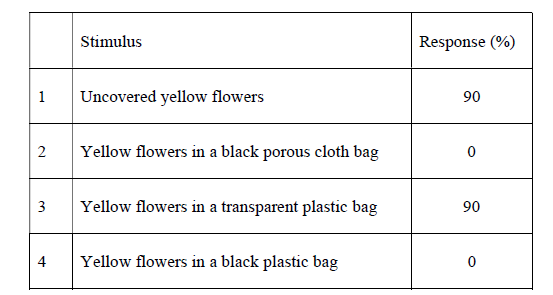
\includegraphics[width=0.5\columnwidth]{figs/15.png}
    \caption{\centering for q-40}
    \label{fig:placeholder_15}
\end{figure}
\hfill \brak{\text{GATE EC 2017}}

\item For the DC analysis of the Common-Emitter amplifier shown in $\figref{fig:placeholder_16}$, neglect the base current and assume that the emitter and collector currents are equal. Given that $V_T = 25$ mV, $V_{BE} = 0.7$ V, and the BJT output resistance $r_o$ is practically infinite. Under these conditions, the midband voltage gain magnitude, $A_v = \sbrak{\frac{v_o}{v_i}}$ in V/V, is
\begin{figure}[H]
    \centering
    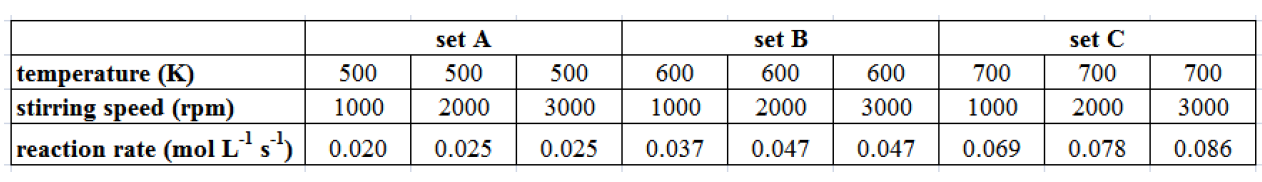
\includegraphics[width=0.5\columnwidth]{figs/16.png}
    \caption{\centering for q-41}
    \label{fig:placeholder_16}
\end{figure}
\hfill \brak{\text{GATE EC 2017}}

\item The amplifier circuit shown in the $\figref{fig:placeholder_17}$ is implemented using a compensated operational amplifier \brak{op-amp}, and has an open-loop voltage gain, $A_0 = 10^5$ V/V and an open-loop cut-off frequency, $f_c = 8$ Hz. The voltage gain of the amplifier at $15$ kHz, in V/V, is
\begin{figure}[H]
    \centering
    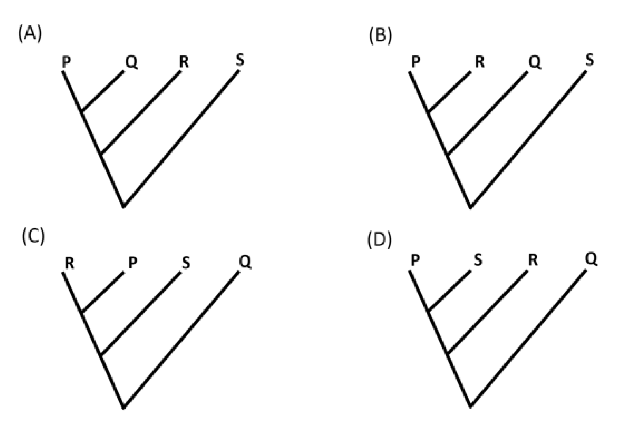
\includegraphics[width=0.3\columnwidth]{figs/17.png}
    \caption{\centering for q-42}
    \label{fig:placeholder_17}
\end{figure}
\hfill \brak{\text{GATE EC 2017}}

\item Which one of the following gives the simplified sum of products expression for the Boolean function $F = m_0 + m_2 + m_3 + m_5$, where $m_0$, $m_2$, $m_3$, and $m_5$ are minterms corresponding to the inputs $A$, $B$, and $C$ with $A$ as the MSB and $C$ as the LSB?
\begin{multicols}{2}
\begin{enumerate}
\item $\overline{A}B + \overline{A}B\overline{C} + A\overline{B}C$
\item $\overline{AC} + \overline{A}B + A\overline{B}C$
\item $\overline{AC} + A\overline{B} + A\overline{B}C$
\item $\overline{A}BC + \overline{AC} + A\overline{B}C$
\end{enumerate}
\end{multicols}
\hfill \brak{\text{GATE EC 2017}}

\item A 4-bit shift register circuit configured for right-shift operation, i.e., $D_{\text{in}} \rightarrow A$, $A \rightarrow B$, $B \rightarrow C$, $C \rightarrow D$, is shown in $\figref{fig:placeholder_18}$. If the present state of the shift register is $ABCD = 1101$, the number of clock cycles required to reach the state $ABCD = 1111$ is $\underline{\hspace{2cm}}$ .
\begin{figure}[H]
    \centering
    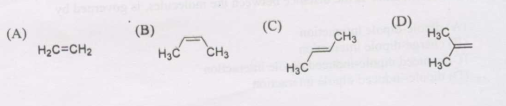
\includegraphics[width=0.3\columnwidth]{figs/18.png}
    \caption{\centering for q-44}
    \label{fig:placeholder_18}
\end{figure}

\hfill \brak{\text{GATE EC 2017}}

\item The following five instructions were executed on an 8085 microprocessor:  
\begin{align*}
MVI A, 33H  
\\ MVI B, 78H
\\ ADD B  
\\ CMA  
\\ ANI 32H  
\end{align*}
The Accumulator value immediately after the execution of the fifth instruction is
\begin{multicols}{4}
\begin{enumerate}
\item $00H$
\item $10H$
\item $11$
\item $32H$
\end{enumerate}
\end{multicols}
\hfill \brak{\text{GATE EC 2017}}

\item A finite state machine \brak{FSM} is implemented using the D flip-flops $A$ and $B$, and logic gates, as shown in the $\figref{fig:placeholder_19}$ below. The four possible states of the FSM are $Q_A Q_B = 00$, $01$, $10$, and $11$. Assume that $X_{\text{IN}}$ is held at a constant logic level throughout the operation of the FSM. When the FSM is initialized to the state $Q_A Q_B = 00$ and clocked, after a few clock cycles, it starts cycling through
\begin{figure}[H]
    \centering
    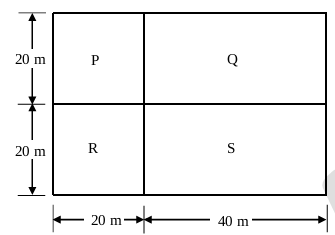
\includegraphics[width=0.5\columnwidth]{figs/19.png}
    \caption{\centering for q-46}
    \label{fig:placeholder_19}
\end{figure}
\begin{multicols}{2}
\begin{enumerate}
\item All of the four possible states if $X_{\text{IN}} = 1$
\item Three of the four possible states if $X_{\text{IN}} = 0$
\item Only two of the four possible states if $X_{\text{IN}} = 1$
\item Only two of the four possible states if $X_{\text{IN}} = 0$
\end{enumerate}
\end{multicols}
\hfill \brak{\text{GATE EC 2017}}

\item A linear time invariant \brak{LTI} system with the transfer function  
$G\brak{s} = \dfrac{K\brak{s+2}\brak{s+3}}{\brak{s+1}\brak{s^2 - 3s + 2}}$  
is connected in unity feedback configuration. For the closed loop system shown, the root locus for $0 < K < \infty$ intersects the imaginary axis for $K = 1.5$. The closed loop system is stable for
\begin{figure}[H]
    \centering
    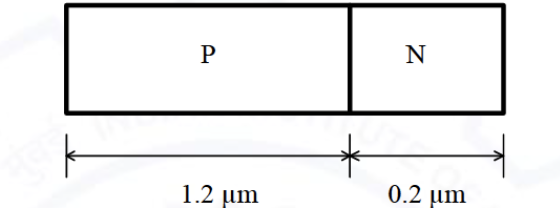
\includegraphics[width=0.5\columnwidth]{figs/20.png}
    \caption{\centering for q-47}
    \label{fig:placeholder_20}
\end{figure}
\begin{multicols}{2}
\begin{enumerate}
\item $K > 1.5$
\item $1 < K \leq 1.5$
\item $0 < K < 1$
\item No positive value of $K$
\end{enumerate}
\end{multicols}
\hfill \brak{\text{GATE EC 2017}}

\item Which one of the following options correctly describes the locations of the roots of the equation $s^4 + s^2 + 1 = 0$ on the complex plane?
\begin{multicols}{2}
\begin{enumerate}
\item Four left half plane \brak{LHP} roots
\item One right half plane \brak{RHP} root, one LHP root and two roots on the imaginary axis
\item Two RHP roots and two LHP roots
\item All four roots are on the imaginary axis
\end{enumerate}
\end{multicols}
\hfill \brak{\text{GATE EC 2017}}

\item The Nyquist plot of the transfer function  
$G\brak{s} = \dfrac{K}{\brak{s^2 + 2s + 2}\brak{s + 2}}$  
does not encircle the point $\brak{-1 + j0}$ for $K = 10$ but does encircle the point $\brak{-1 + j0}$ for $K = 100$. Then the closed loop system \brak{\text{having unity gain feedback}} is
\begin{multicols}{2}
\begin{enumerate}
\item Stable for $K = 10$ and stable for $K = 100$
\item Stable for $K = 10$ and unstable for $K = 100$
\item Unstable for $K = 10$ and stable for $K = 100$
\item Unstable for $K = 10$ and unstable for $K = 100$
\end{enumerate}
\end{multicols}
\hfill \brak{\text{GATE EC 2017}}

\item In binary frequency shift keying \brak{FSK}, the given signal waveforms are  
$u_0\brak{t} = 5 \cos\brak{20000\pi t}$ for $0 < t < T$  
$u_1\brak{t} = 5 \cos\brak{22000\pi t}$ for $0 < t < T$  
where $T$ is the bit-duration interval and $t$ is in seconds. Both $u_0\brak{t}$ and $u_1\brak{t}$ are zero outside the interval $0 \leq t \leq T$. With a matched filter \brak{correlator} based receiver, the smallest positive value of $T$ \brak{\text{in milliseconds}} required to have $u_0\brak{t}$ and $u_1\brak{t}$ uncorrelated is
\begin{multicols}{4}
\begin{enumerate}
\item $0.25ms$
\item $0.5ms$
\item $0.75ms$
\item $1.0ms$
\end{enumerate}
\end{multicols}
\hfill \brak{\text{GATE EC 2017}}

\item Let $X\brak{t}$ be a wide sense stationary random process with the power spectral density $S_X\brak{f} = e^{-|f|}$, where $f$ is in Hz. The random process $X\brak{t}$ is input to an ideal lowpass filter with frequency response  
$H\brak{f} = \begin{cases}
1, & |f| \leq \frac{1}{2} \\
0, & |f| > \frac{1}{2}
\end{cases}$  

The output of the lowpass filter is $Y\brak{t}$. 
\begin{figure}[H]
    \centering
    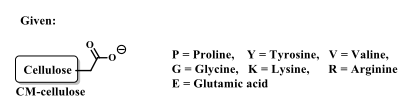
\includegraphics[width=0.5\columnwidth]{figs/21.png}
    \caption{\centering for q-51}
    \label{fig:placeholder_21}
\end{figure}
Let $E$ be the expectation operator. Consider the following statements:  
\begin{enumerate}[label=\Roman*.]
    \item $E\brak{X\brak{t}} = E\brak{Y\brak{t}}$ 
    \item $E\brak{X^2\brak{t}} = E\brak{Y^2\brak{t}}$  
    \item $E\brak{Y^2\brak{t}} = 2$  
\end{enumerate}
Select the correct option:  
\begin{multicols}{2}
\begin{enumerate}
\item Only I is true
\item Only II and III are true
\item Only I and II are true
\item Only I and III are true
\end{enumerate}
\end{multicols}
\hfill \brak{\text{GATE EC 2017}}

\item A continuous time signal $x\brak{t} = 4 \cos\brak{200\pi t} + 8 \cos\brak{400\pi t}$ is the input to a linear time invariant \brak{LTI} filter with the impulse response  
$h\brak{t} = \begin{cases}
-2 \sin\brak{300\pi t}/600, & t \neq 0 \\
1, & t = 0
\end{cases}$  
Let $y\brak{t}$ be the output of this filter. The maximum value of $|y\brak{t}|$ is
\begin{multicols}{4}
\begin{enumerate}
\item $7.9$
\item $8.0$
\item $8.1$
\item $8.2$
\end{enumerate}
\end{multicols}
\hfill \brak{\text{GATE EC 2017}}

\item An optical fiber is kept along the $z$ direction. The refractive indices for the electric fields along $x$ and $y$ directions in the fiber are $n_x = 1.5000$ and $n_y = 1.5001$, respectively. The free space wavelength of a light wave propagating in the fiber is $1.5$ $\mu$m. If the lightwave is circularly polarized at the input of the fiber, the minimum propagation distance after which it becomes linearly polarized, in centimetres, is
\begin{multicols}{4}
\begin{enumerate}
\item $0.36$
\item $0.37$
\item $0.38$
\item $0.39$
\end{enumerate}
\end{multicols}
\hfill \brak{\text{GATE EC 2017}}

\item The expression for an electric field in free space is  
$E = E_0 \brak{x + y + j2z} e^{-j\brak{\omega t - kx + ky}}$  
This electric field
\begin{enumerate}
\item Does not represent a plane wave
\item Represents a circularly polarized plane wave propagating normal to the $z$-axis
\item Represents an elliptically polarized plane wave propagating along the $x$-$y$ plane
\item Represents a linearly polarized plane wave
\end{enumerate}
\hfill \brak{\text{GATE EC 2017}}

\item A half wavelength dipole is kept in the $x$-$y$ plane and oriented along $45^\circ$ from the $x$-axis. Determine the direction of null in the radiation pattern for $0 \leq \theta \leq \pi$. Here the angle $\theta$ is measured from the $z$-axis, and the angle $\phi$ is measured from the $x$-axis in the $x$-$y$ plane.
\begin{multicols}{2}
\begin{enumerate}
\item $\theta = 90^\circ$, $\phi = 45^\circ$
\item $\theta = 45^\circ$, $\phi = 90^\circ$
\item $\theta = 90^\circ$, $\phi = 135^\circ$
\item $\theta = 45^\circ$, $\phi = 135^\circ$
\end{enumerate}
\end{multicols}
\hfill \brak{\text{GATE EC 2017}}

\item She has a sharp tongue and it can occasionally turn
\begin{multicols}{4}
\begin{enumerate}
\item Hurtful
\item Left
\item Methodical
\item Vital
\end{enumerate}
\end{multicols}
\hfill \brak{\text{GATE EC 2017}}

\item I $\underline{\hspace{0.5cm}}$ made arrangements had I $\underline{\hspace{0.5cm}}$ informed earlier.
\begin{multicols}{2}
\begin{enumerate}
\item Could have, been
\item Would have, being
\item Had, have
\item Had been, been
\end{enumerate}
\end{multicols}
\hfill \brak{\text{GATE EC 2017}}

\item In the summer, water consumption is known to decrease overall by $25\%$. A Water Board official states that in the summer household consumption decreases by $20\%$, while other consumption increases by $70\%$. Which of the following statements is correct?
\begin{enumerate}
\item The ratio of household to other consumption is $8/17$
\item The ratio of household to other consumption is $1/17$
\item The ratio of household to other consumption is $17/8$
\item There are errors in the official's statement
\end{enumerate}
\hfill \brak{\text{GATE EC 2017}}

\item $40\%$ of deaths on city roads may be attributed to drunken driving. The number of degrees needed to represent this as a slice of a pie chart is
\begin{multicols}{4}
\begin{enumerate}
\item $120$
\item $144$
\item $160$
\item $212$
\end{enumerate}
\end{multicols}
\hfill \brak{\text{GATE EC 2017}}

\item Some tables are shelves. Some shelves are chairs. All chairs are benches. Which of the following conclusions can be deduced from the preceding sentences?
\begin{enumerate}[label=\roman*.]
\item At least one bench is a table
\item At least one shelf is a bench
\item At least one chair is a table
\item All benches are chairs
\end{enumerate}
\begin{enumerate}
    \item Only i
    \item Only ii
    \item Only ii and iii
    \item Only iv
\end{enumerate}
\hfill \brak{\text{GATE EC 2017}}

\item "If you are looking for a history of India, or for an account of the rise and fall of the British Raj, or for the reason of the cleaving of the subcontinent into two mutually antagonistic parts and the effects this mutilation will have in the respective sections, and ultimately on Asia, you will not find it in these pages; for though I have spent a lifetime in the country. I lived too near the seat of events, and was too intimately associated with the actors, to get the perspective needed for the impartial recording of these matters". 
Here, the word 'antagonistic' is closest in meaning to 
\begin{multicols}{4}
\begin{enumerate}
\item Impartial
\item Argumentative
\item Separated
\item Hostile
\end{enumerate}
\end{multicols}
\hfill \brak{\text{GATE EC 2017}}

\item $S, T, U, V, W, X, Y, Z$ are seated around a circular table. $T$'s neighbours are $Y$ and $V$. $Z$ is seated third to the left of $T$ and second to the right of $S$. $U$'s neighbours are $S$ and $Y$; and $T$ and $W$ are not seated opposite each other. Who is third to the left of $V$?
\begin{multicols}{4}
\begin{enumerate}
\item $X$
\item $W$
\item $U$
\item $T$
\end{enumerate}
\end{multicols}
\hfill \brak{\text{GATE EC 2017}}

\item Trucks \brak{\text{10 m long}} and cars \brak{\text{5 m long}} go on a single lane bridge. There must be a gap of at least $20$ m after each truck and a gap of at least $15$ m after each car. Trucks and cars travel at a speed of $36$ km/h. If cars and trucks go alternately, what is the maximum number of vehicles that can use the bridge in one hour?
\begin{multicols}{4}
\begin{enumerate}
\item $1440$
\item $1200$
\item $720$
\item $600$

\end{enumerate}
\end{multicols}
\hfill \brak{\text{GATE EC 2017}}

\item There are 3 Indians and 3 Chinese in a group of 6 people. How many subgroups of this group can we choose so that every subgroup has at least 1 Indian?
\begin{multicols}{4}
    \begin{enumerate}
        \item $56$
        \item $52$
        \item $48$
        \item $44$
    \end{enumerate}
\end{multicols}
\hfill \brak{\text{GATE EC 2017}}

\item A contour line joins locations having the same height above the mean sea level. The following is a contour plot of a geographical region. Contour lines are shown at 25m intervals  in this plot .
\begin{figure}[H]
    \centering
    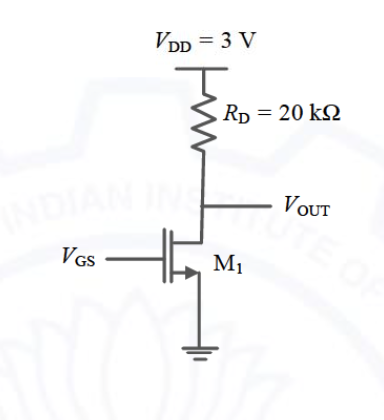
\includegraphics[width=0.5\columnwidth]{figs/22.png}
    \caption{\centering for q-65}
    \label{fig:placeholder_22}
\end{figure}
The path is from P to Q is best described by 
\begin{multicols}{2}
    \begin{enumerate}
        \item Up-Down-Up-Down
        \item Down-Up-Down-Up
        \item Down-Up-Down
        \item Up-Down-Up
    \end{enumerate}
\end{multicols}
\hfill \brak{\text{GATE EC 2017}}

\end{enumerate}
\end{document}
